% Left frame
%%%%%%%%%%%%%%%%%%%%
\begin{figure}
	\hfill
	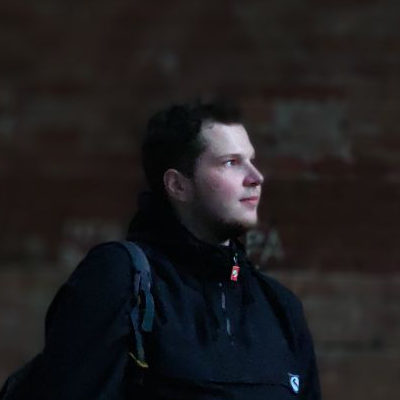
\includegraphics[width=0.6\columnwidth]{photo}
	\vspace{-7cm}
\end{figure}

\begin{flushright}\small

\end{flushright}\normalsize
\framebreak


% Right frame
%%%%%%%%%%%%%%%%%%%%
\Huge\bfseries {{\color{Cyan} Ilya} {\color{Black} Chesalin}} \\
\Large\bfseries Student, programmer, hacker \\

\normalsize\normalfont

% About me
I was born in Ryazan, Russia, and I have been passionate about information
technologies for most of my life.

Since school, I was always amazed at how complicated and chaotic, on one hand, and how beautiful and organized, on the other hand, the world around us is. It lead me to want to learn maths - the language of nature. This language got applied to physics, which to this day amazes me.

At some point, my vector of focus changed to information technologies. I started to learn how computers work, and I learn something every single day. I still apply this knowledge daily for creating better and more optimized software and for hacking the technology around me, for creating a better world to live in.

\Sep

% Skills
\CVSection{Skills}

\CVItem{Languages I speak}
\begin{multicols}{3}
\begin{compactitem}[\color{Cyan}$\circ$]
    \item Russian, native
    \item English, B2
\end{compactitem}
\end{multicols}

\SmallSep

\CVItem{Platforms}
\begin{multicols}{3}
\begin{compactitem}[\color{Cyan}$\circ$]
	\item Windows 10
	\item Arch Linux
	\item Debian / Ubuntu
	\item Kali Linux
	\item \ldots
\end{compactitem}
\end{multicols}

\SmallSep

\CVItem{Programming and other Languages}
\begin{multicols}{3}
\begin{compactitem}[\color{Cyan}$\circ$]
    \item Python
    \item Bash/Zsh
	\item C
    \item C++
    \item Object Pascal
    \item HTML and CSS
    \item JavaScript
    \item SQL
    \item \LaTeX
	\item \ldots
\end{compactitem}
\end{multicols}

\SmallSep

\CVItem{Technologies}
\begin{multicols}{3}
\begin{compactitem}[\color{Cyan}$\circ$]
    \item Open Source \heart\
    \item Git
    \item Qt
    \item GDB
    \item Valgrind
    \item x86dbg / x64dbg
    \item NodeJS
    \item VueJS
    \item MongoDB
    \item PostgreSQL
    \item Visual Studio Code
    \item vim
    \item \ldots
\end{compactitem}
\end{multicols}

\Sep

% Experience
\CVSection{Experience}

\CVItem{October 2018 - present} \\
at \textit{D-Link, Russia}
as \textit{full-stack software engineer}
\SmallSep

In October, I was transferred to another project, where I do front-end and back-end development.
\SmallSep

\texttt{Linux / JavaScript / NodeJS / VueJS / MongoDB}

\SmallSep

\CVItem{November 2018 - September 2019} \\
at \textit{D-Link, Russia}
as \textit{system engineer}
\SmallSep

After taking cources on "Linux Embedded Programming Fundamentals" in 2017-2018, I got opportunity to join D-Link Developer team.
\SmallSep

\texttt{Linux / C / GDB / Valgrind}

\clearpage
\framebreak
\framebreak

\CVItem{July 2017 - August 2017, July 2018 - August 2018} \\
at \textit{Svyaztransneft, JSC, Oka Region Industrial Communication Directorate}
as \textit{2nd grade techician}
\SmallSep

In the Summer of 2017, during study break, I had the opportunity to work part-time. In the Summer of 2018 I was invited back.

\Sep

% Education
\CVSection{Education}
\CVItem{2016 - present} \\
at \textit{Ryazan State Radio Engineering University after V. Utkin}
\SmallSep

Since 2016, I have been a student at RSREU, at the departament of Information Security of the Faculty of Computer Engineering.

My speciality is Information Security of Automated Systems.

\SmallSep

\CVItem{2013 - 2016} \\
at \textit{Correspondence School of Physics and Technology of The Moscow Institute of Physics and Technology}
\SmallSep

Since ninth grade, I studied on programs of continuing education of a scientific and technical orientation.

\SmallSep

\CVItem{2005 - 2016} \\
at \textit{School 39 - Center of physical and mathematical eduation}
\SmallSep

At school I was passionate about mathematics and physics, taking part in lots of olympiads by Rosatom, MEPhI, URFO and many others.

\Sep

% Hackathons
\CVSection{Hackathons}

\CVItem{WebPurple Codenjoy} \\
by \textit{Webpurple, Ryazan}
on \textit{14 July 2018}
\SmallSep

My first ever hackathon was in Ryazan, and it was just 4 hours.

The aim was to write a bot to play tetris. Even though it was my first encounter with JavaScript, I managed to take 4th place.
\SmallSep

\texttt{JavaScript / Codenjoy}

\Sep

% Contacts
\CVSection{Contacts}

\CVItem{Email} \\
\url{evilyach@protonmail.com}

\CVItem{Github} \\
\url{github.com/evilyach}

\SmallSep